\documentclass[10pt]{beamer}
\usetheme[
%%% options passed to the outer theme
%    progressstyle=movCircCnt,   %either fixedCircCnt, movCircCnt, or corner
%    rotationcw,          % change the rotation direction from counter-clockwise to clockwise
%    shownavsym          % show the navigation symbols
  ]{AAUsimple}
  
% If you want to change the colors of the various elements in the theme, edit and uncomment the following lines
% Change the bar and sidebar colors:
%\setbeamercolor{AAUsimple}{fg=red!20,bg=red}
%\setbeamercolor{sidebar}{bg=red!20}
% Change the color of the structural elements:
%\setbeamercolor{structure}{fg=red}
% Change the frame title text color:
%\setbeamercolor{frametitle}{fg=blue}
% Change the normal text color background:
%\setbeamercolor{normal text}{fg=black,bg=gray!10}
% ... and you can of course change a lot more - see the beamer user manual.

\usepackage[utf8]{inputenc}
\usepackage[english]{babel}
\usepackage[T1]{fontenc}
% Or whatever. Note that the encoding and the font should match. If T1
% does not look nice, try deleting the line with the fontenc.
\usepackage{helvet}
\usepackage[citestyle=verbose,sorting=none,
            bibencoding=inputenc,backend=bibtex]{biblatex}
\addbibresource{refs.bib}
\usepackage{url}
% colored hyperlinks
\newcommand{\chref}[2]{%
  \href{#1}{{\usebeamercolor[bg]{AAUsimple}#2}}%
}

\title{Visualization Fundamentals}

% \subtitle{}  % could also be a conference name

\date{\today}

\author{
  Tobias Jensen
  \href{mailto:tlj@its.aau.dk}{{\tt tlj@its.aau.dk}} \\
}

\institute[
%  {\includegraphics[scale=0.2]{aau_segl}}\\ %insert a company, department or university logo
  Aalborg University\\
  Denmark
] % optional - is placed in the bottom of the sidebar on every slide
{% is placed on the bottom of the title page
  Aalborg University\\
  Denmark
  
  %there must be an empty line above this line - otherwise some unwanted space is added between the university and the country (I do not know why;( )
}

% specify a logo on the titlepage (you can specify additional logos an include them in 
% institute command below
\pgfdeclareimage[height=1.5cm]{titlepagelogo}{AAUgraphics/aau_logo_new} % placed on the title page
%\pgfdeclareimage[height=1.5cm]{titlepagelogo2}{AAUgraphics/aau_logo_new} % placed on the title page
\titlegraphic{% is placed on the bottom of the title page
  \pgfuseimage{titlepagelogo}
%  \hspace{1cm}\pgfuseimage{titlepagelogo2}
}

\begin{document}
% the titlepage
{\aauwavesbg%
\begin{frame}[plain,noframenumbering] % the plain option removes the header from the title page
  \titlepage
\end{frame}}

%%%%%%%%%%%%%%%%

% TOC
%\begin{frame}{Agenda}{}
%\tableofcontents
%\end{frame}

%%%%%%%%%%%%%%%%

\begin{frame}{Data types}{}

  \scriptsize
  \begin{tabular}{|p{2.7cm}|p{2cm}|p{2cm}|p{3cm}|} \hline \hline
    Type & Examples & Appropriate scale & Description \\ \hline
Quantitative/numerical continuous & 1.2, $4.2*10^{30}$, 83 & Continuous & Integer, real, complex \\ \hline
Quantitative/numerical discrete & 1,2,3,4             & Discrete   & Mostly integers, but also as a result of mapping real to discrete \\ \hline
Qualitative/categorical unordered & bed/milk/bourbon, urban/rural & Discrete & No inherent order. Also called factors \\ \hline
Qualitative/categorical ordered & good/fair/poor & Discrete & Also called ordered factors \\ \hline
Date or time                    & 10.00, Oct. 10 1981 & Continuous or discrete & \\ \hline
Text                            & Hello to the world  & None or discrete & Free-form. Can be treated as discrete \\\hline \hline
\end{tabular}
\end{frame}

%%%%%%%%%%%%%%%%

\begin{frame}{Aestetics}{Position}
\centering  Examples: Cartesian and polar coordinate systems\\[2em]
  \centering 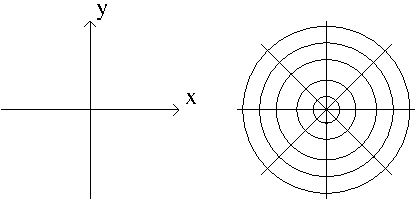
\includegraphics[width=0.7\textwidth]{pics/position.pdf}
  \\[2em]
  Continuous or discrete data
\end{frame}

%%%%%%%%%%%%%%%%

\begin{frame}{Aestetics}{Shape}
  \centering 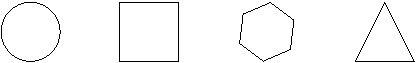
\includegraphics[width=0.7\textwidth]{pics/shape.pdf}
  \\[2em]
  Discrete data
\end{frame}

%%%%%%%%%%%%%%%%

\begin{frame}{Aestetics}{Size}
  \centering 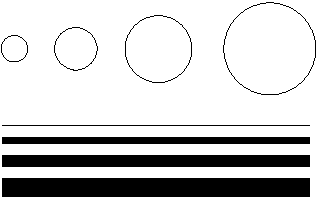
\includegraphics[width=0.7\textwidth]{pics/size.pdf}
  \\[2em]
  Continuous or discrete data
\end{frame}

%%%%%%%%%%%%%%%%

\begin{frame}{Aestetics}{Color}
  \centering 
\includegraphics[width=0.7\textwidth]{pics/color.pdf}
  \\[2em]
  Continuous (gradient) and discrete data
\end{frame}

%%%%%%%%%%%%%%%%

\begin{frame}{Aestetics}{Line types}
  \centering 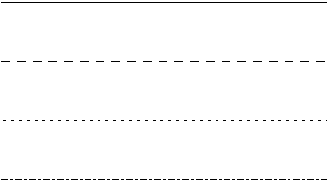
\includegraphics[width=0.7\textwidth]{pics/line_types.pdf}
  \\[2em]
  Discrete data
\end{frame}

%%%%%%%%%%%%%%%%

\begin{frame}{Aestetics}{Additional as often used in visualization terminology}
  \begin{itemize}
     \item alpha (transparency)
     \item stroke (width of boundary of object)
     \item color (color of boundary of object)
     \item fill (color or pattern inside object)
  \end{itemize}
  \centering 
\includegraphics[width=0.7\textwidth]{pics/combi.pdf}
\end{frame}

%%%%%%%%%%%%%%%%

\begin{frame}{Talking about visualization}{}
   \begin{itemize}
     \item[ugly]—A figure that has aesthetic problems but otherwise is clear and informative.
     \item[bad]—A figure that has problems related to perception; it may be unclear, confusing, overly complicated, or deceiving.
     \item[wrong]—A figure that has problems related to mathematics; it is objectively incorrect.
   \end{itemize}
\end{frame}

\begin{frame}{Reference}{}

  Claus O. Wilke\\
  Fundamentals of Data Visualization\\
  \url{https://serialmentor.com/dataviz/index.html}

\end{frame}
%%%%%%%%%%%%%%%

\end{document}
